
%%%%%%%%%%%%%%%%%%%%%%%%%%%%%%%%%%%%%%%%%%%%%%%%%%%%%%%%%%%%%%%%%%% 
%                                                                 %
%                           INTRODUCTION                          %
%                                                                 %
%%%%%%%%%%%%%%%%%%%%%%%%%%%%%%%%%%%%%%%%%%%%%%%%%%%%%%%%%%%%%%%%%%% 
 
\chapter{INTRODUCTION}
\label{chapter:intro}

% magical first sentence
% explain like you would to your parents/non-technological people
% - explain how keyframe animation currently works
% explain in more technical terms what this means
% - problems with current techniques
% - what can be done (auto animation)
% - overview of controllers
% - overview of the technique
Animations of human characters are used heavily in video games, movies, and other fields.  Especially with the increasing usage of complex environment traversal in both film and video games, many similar animations of athletic motions must be created with small changes to tune the motion to the particular situation, environment, and character.  Creation of such animations is largely done by hand by artists, posing the character for each time step of the animation.  In 2D animation this takes the form of an animation cel, also referred to as sprite sheets in 2D computer animation, as shown in Figure \ref{fig:sprite_sheet}.  These sprites may be drawn by hand or generated through 3D models.

Artists will frequently use a method called keyframing, which originated in 2D animation but was later applied to 3D animation with some modifications.  In a keyframe animation, certain ``key'' parts of the animated sequence are specified, with the remaining frames filled in in a process called "in betweening or ``tweening,'' using an automated interpolation method or manual frame addition.  For 2D animation, the artist will need to generate the intermediate images themselves or have a program interpolate between images.  In 3D, keyframe animations are performed on a 3D model, storing transformation data about the model for each frame and playing back the animation by repeating the transformations, interpolating between them to produce smooth animations.

% figure of sprite animation frames
\begin{figure}[htp]
    \centering
    \includegraphics[width=\textwidth]{images/sprite_example/platformer_sprites_jump.png}
    \includegraphics[width=\textwidth]{images/sprite_example/platformer_sprites_walk.png}
    \caption[Example of a 2D Sprite Animation]{A 2D sprite sheet used to produce a jumping animation (top row) and a walking animation (bottom row) for a stick figure character.  The frames in this case are laid out in a single image for demonstration purposes, progressing in order starting with frame 0, the frame farthest left in this sprite sheet.  An artist may create keyframes and then fill in intermediary poses to produce a full sprite sheet as above.  These sprite sheets were created by Clint Bellanger using a 3D model and are licensed under Creative Commons Attribution 3.0, retrieved from opengameart.org.}
    \label{fig:sprite_sheet}
\end{figure}

%3D models are described as a mesh, a collection of primitive polygons (i.e. quadrilaterals or triangles) which are stored as vertices.  This mesh describes what is drawn, including any texture, color, and other material information.  Along with the mesh, a skeleton, or rig, is stored.  The rig describes a hierarchical structure of bones and accompanying joints.  Each vertex is given a series of weights describing the impact each joint has on its transformation.  This allows many vertices, and therefore many polygons, to be transformed at once in organized groups, simplifying the problem of animating the model to a matter of transforming the skeleton in the desired manner.  To animate this 3D model, an artist specifies key frames of the animation by positioning the skeleton at different time steps.  The stored key frames, instead of an image, are the transformations of each joint at this frame or step of the animation, which a rendering or game engine can interpolate between to produce the final result.

Specifying these animation frames is work intensive, taking up significant time and resources to produce for a single character.  Additionally, similar animations may need to be produced for slightly different scenarios, with only minor modifications required.  These minor modifications can be made to fit a different setting, such as a character jumping on Earth or on the moon, or can be for different characters, such as a large person moving in contrast with a small child.  Though the movement itself may be similar, manual changes must be made, requiring artist time which could be spent generating new assets.  

Recent work in animation generation seeks to automate this process, replacing the manual process with a procedural one.  Physics-based simulations can be used to produce controllers for the skeleton, determining joint positions and rotations for keyframes automatically.  Not only does this reduce the effort involved in the creation process, but this also provides a basis for dynamic interaction between a character's animation and the environment.  With manual keyframe animations this is not possible, as any specific interaction between a character and the environment must be manually created by an animator 

I present a controller that takes a skeleton as input, with additional parameters describing the character.  I then simulate a jumping motion on the character, determining a sequence of poses based on the character's muscles to produce a keyframe animation.  The additional character parameters describe the character's mass, muscles, the constraints placed on each joint to prevent unnatural rotations, and a description of the jump indicating desired time and distance.  Mass is specified per-limb, with each mass stored in the joint object affecting the limb to allow for calculation of the character's center of mass.  

\newcommand{\frameimage}[1]{\fbox{\includegraphics[scale=1.0]{#1}}}

\begin{figure}[htp]
	\centering
	\begin{subfigure}[h]{0.16\textwidth}
		\frameimage{images/jump_stages/ps1_windup.png}
		\caption{Windup}
	\end{subfigure}
	\begin{subfigure}[h]{0.32\textwidth}
		\frameimage{images/jump_stages/ps2_takeoff.png}
		\caption{Takeoff}
	\end{subfigure}
	\begin{subfigure}[h]{0.48\textwidth}
		\frameimage{images/jump_stages/ps3_airborne.png}
		\caption{In-Air}
	\end{subfigure}
	%\includegraphics[width=\textwidth]{images/jump_stages/jump_stages.png}
	\caption[Example of stages of jumping]{An example 2D sprite animation of a simple human character jumping, with the jump divided into the windup, takeoff, and in-air stages.  A landing is absent from this sequence.  The windup consists of a short crouch to prepare for the jump, creating an opportunity for the body to extend and thus accelerate.  The takeoff performs this acceleration, shifting its center of mass forward past its feet and the character becomes airborne.  During the in-air phase the character moves its body to control the fall, in this case spreading its arms and shifting its feet from behind its pelvis to in front of its pelvis.}
	\label{fig:jumpStages}
\end{figure}

I divide a jump into five stages: path estimation, windup, thrust, in air maneuvering, and landing. My controller works with the initial path estimation, windup, and thrust stages of the motion as shown in Figure \ref{fig:jumpStages}.  Poses are  calculated by modeling muscles as Hookean springs attached to the skeleton at 2 points and crossing a joint as shown in Figure \ref{fig:forceCalc}. Spring constants for the muscles are specified by the user, allowing my simulation to animate characters of various strengths and body makeups.  Spring displacement from rest is calculated using the bend in the joint and constants describing the skeleton.  Using the spring displacement, a particular pose of a joint is related to the usage of the character's muscle and the elasticity of the connective tissue of the muscle and joint.

\begin{figure}[ht]
	\centering
	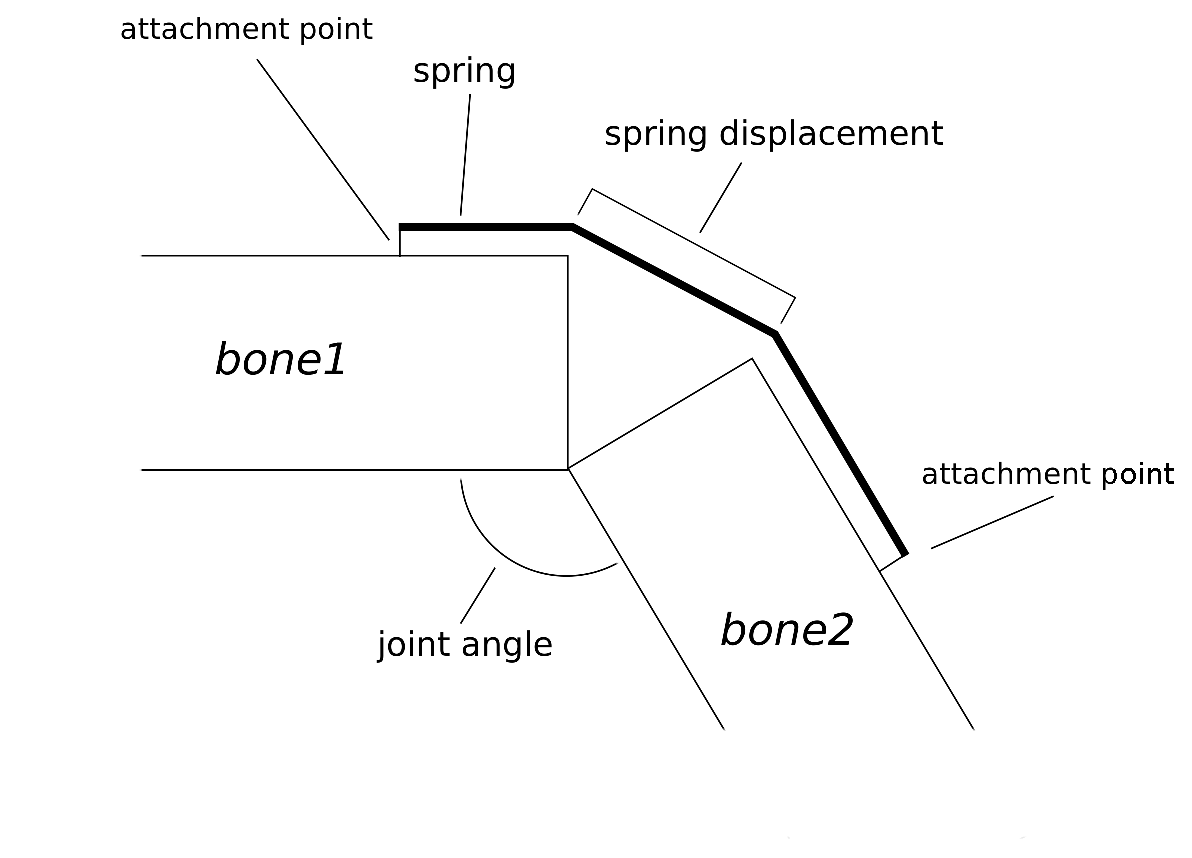
\includegraphics[width=10cm]{images/spring_calc/spring_angle_calc.eps}
	\caption[Diagram of muscle setup]{Visual representation of the setup of bones and muscles for a single joint.  This illustrates the method by which I calculate the spring displacement, taking the bones as rigid blocks which separate and stretch the string as the joint bends.}
	\label{fig:forceCalc}
\end{figure}

Two approaches are described in this thesis, one using torque and one using elastic energy.  As the springs contract, they produce forces on the bones, which result in torques at each joint.  These torques are then used to calculate a windup pose for the character by calculating resultant linear acceleration for the character's center of mass, which is compared to a calculated necessary acceleration to make the jump.  This linear acceleration is then used to compute the motion of the takeoff and in-air phases of the jump, which are sampled to create frames of an animation.  

The second approach uses the spring displacement to calculate the elastic potential energy of each muscle, which is modeled by a single linear spring.  By assuming perfect conservation of energy, I compare the total elastic potential energy of the character's muscles to a calculated necessary kinetic energy for the jump to be completed.

To control the motion and maintain plausibility, I calculate the character's center of mass and supporting polygon each frame.  This allows the character to maintain balance while flexing its joints, the position of the character's joints are adjusted to keep the center of mass positioned over the supporting polygon.  While flexing, the character constantly checks the position of its center of mass against the calculated supporting polygon, ensuring the center of mass is over the support and as close to the center as possible.

I use an inverse kinematic solver to help determine poses of intermediate joints.  This allows me to find the necessary pose for the ankle and knee of the character given the position of its foot and hip.  Many solutions in this region are possible, so I constrain the skeleton such that only those poses where the joints are within human ranges of motion are possible.

The next stage of the motion is the thrust stage where the character releases from the ground by using the potential energy of the spring-muscles to accelerate its center of mass upward.  This is handled by applying the calculated accelerations from the windup stage to the character's pelvis to accelerate the center of mass, with the inverse kinematic solver determining the poses of the legs as they unbend.  Balance must be maintained, and the relative rate of rotation of the different joints of the leg must be balanced with each other to maintain foot position while the body is transformed.  As the skeleton is a tree with its root at the character's pelvis, this can be a challenge, necessitating the use of the inverse kinematics solver.  Due to the nature of the inverse kinematics algorithm used, the extension propagates from the hip to the feet.  

The character then proceeds through the in-air portion of the jump, where the acceleration changes due to gravity before they finally land.  I assume a simple trajectory for the in-air phase, though more complex motions with turns, flips, or interaction with the environment could be created.  My simulation ends when the character's feet contact the ground, ending the in-air phase.  Other work, such as that by \liufall, has handled landing and creating a separate controller to handle this is beyond the scope of this thesis \cite{falling_landing}.

My controller is made to be a module, able to be used with other controllers as part of a larger system.  Its modularity takes the form of detecting and handling its state at each stage, consisting of its position, velocity, acceleration, pose, muscle state, and any collisions or forces applied. The controller performs actions when it has a response to its current state and ends control when it no longer has an appropriate response to allow a separate controller to handle the situation.  This allows each controller to do a smaller job well, and to act as a portion of a larger state machine handling a character's actions. Several such controllers can be connected to produce more complex animations or animation sequences, utilizing bounded starting and finishing conditions for the character as well as bounds on expected conditions during operation to allow handling of stimuli during operation.

% figure of current keyframe animation process in maya
% accompanying video for presentation
% accompanying figure/video of the resulting animation in 3d

 
\section{A Description of 3D Animation Creation}
\label{section:anim_ex}
To motivate the necessity for an automated animation method, I present an example of the method for producing an animation by hand.  First a mesh and rig must be produced, which I also require for my simulation.  This is a time and skill intensive process, requiring the artist to exercise their technical and creative knowledge and ability to create the character's figure, the mesh, and to create and attach a skeleton, the rig.  

A mesh is constructed of faces which are in turn made of vertices, and each vertex must be assigned a weight for each joint of the rig to indicate the way the vertex should transform when the joint in the rig is transformed.  These joints serve not only as a joint in the anatomical sense, but as a tracked point in the skeleton.  The joints are connected by bones, but the information is stored at the joint, which sometimes necessitates a joint to be placed in a non-anatomical way.  For example, in my rig I have a joint placed at the head, which not only allows me to rotate the head but tracks the position.  A similar situation arises with the toe and heel, where a joint is used to facilitate the placement of a connecting bone.  Once the mesh and rig are created and the weights for the rig are assigned to the mesh, an animator may create controls to manipulate several joints at once, such as creating a controller to facilitate grasping motions in which many bones of the hand must be manipulated at once.  These controls are formed from an object such as a simple spline to which several joints are constrained, allowing movement of several joints through manipulation of the control object.

Once the rig and mesh are set up, an animator must manipulate the mesh to pose the model.  Study of real subjects may be used to help ensure realism.  For a jumping motion the animator would need to decide how they want to start the animation to allow blending from other movements such as walking, running, or standing.  They must then position the model and record a keyframe.  Keyframes are hand-created frames of the animation which a renderer or game engine may interpolate between to produce a final animation, allowing an animator to create and store few frames, while still creating a smooth animation in the final setting.  This allows few frames to be stored to produce any frame rate of animation, while also reducing the storage requirements in exchange for a minor increase in computation, which is an extra interpolation for each joint in the character.

While the key frames can be sparse and there are tools for aiding in generation, this process requires heavy manual input for each animation for each character, as well as prior knowledge of the motion to be produced.  Characters that move differently due to differences in weight or body makeup must be animated separately, requiring an artist to perform similar, time consuming work.  For example, a character with extremely strong legs may bend less, applying the same force as a weaker character over a shorter distance to achieve the same acceleration.  A heavier character would need to apply much more force to achieve the same acceleration and thus jump height as a lighter character, necessitating stronger muscles or a greater distance over which the force is applied, thus requiring a deeper squat than the light character.  With a simulation-based approach this work could be reduced, especially repeated work, to setting variables such as weight, height, and musculature for the different characters and generating the set of animations desired.  As techniques and technologies improve, a simulation could be used in place of a stored key frame animation, creating the animation in place based on its environment and situation, thus shifting the burden on an animator from preparing poses and keyframes to adjusting body dimensions, weight, strength, and constraints.

For a jump specifically, a human loads the muscles in their legs, quickly moving to a particular bend based on the feedback they feel in their muscles and joints, as well as balance feedback and their knowledge of the jumps they have performed in the past.  The appearance of bearing and lifting weight is difficult to achieve, as the animator must visually match the poses to their knowledge of bodies or to a visual of a similar human to their character performing the motion.  Simulation allows a computer to calculate movement based on physical aspects of the character, incorporating knowledge such as the character's weight and body make up, allowing an animator to produce animations of unfamiliar motions with a higher degree of physical plausibility.

% explain contributions
% - what is the contribution of this technique
% - Unity3D -> what am I getting from outside sources
% - what am I making myself

\section{Contributions}
\label{section:contributions}
	This thesis describes a controller which simulates a jumping motion of a character.  The generated animation is created to be plausible in appearance, using a simplified physical representation.  I sacrifice some physical accuracy in favor of speed and simplicity of creating, describing, and implementing the simulation.  Specifically, I contribute a description for the windup, thrust, and in air phases of a jump and created a controller using a physical simulation and an implementation in \unity{}.  In short, my contributions are:
	\begin{itemize}
		\item A controller which simulates a windup and thrust phase of a jump, moving the character from the ground into the air
		\item A description of character poses based on torque generated by muscles
		\item A description of character poses based on elastic energy of the muscles
		\item A sampling-based method for choosing a pose given muscles and a desired output
		%\item Estimates and quantification of ``good'' values for spring constants
		\item Visualizations of the animations and values for analysis and presentation
	\end{itemize}

\section{Summary}
\label{section:intro_summary}
In this chapter, I introduced the problem of animating a character to perform a jump motion and the simulation-based approach to animation.  I then presented an example of a current method of creating animations in Section \ref{section:anim_ex}, describing how an artist would create a character and animate it for a video game or film.  I then gave a summary of the contributions of this thesis.

Expanding on the ideas introduced in this chapter, Chapter \ref{chapter:previous_work} discusses existing work in simulation, motion capture, and inverse kinematics which inspired and directed the work of this thesis.  Chapter \ref{chapter:animation} discusses my method, describing the torque-based and energy-based simulations I used to produce animations.  Visualization for debugging, understanding, and presenting these animations is discussed in Chapter \ref{chapter:visualization}, and the results themselves are discussed in Chapter \ref{chapter:results}. Lastly, I discuss future work and draw final conclusions in Chapter \ref{chapter:future_work}.